% !Tex program = pdflatex
% 第 2 章: 向量空间
\ifx\allfiles\undefined
\documentclass{note}
\begin{document}
\fi
\chapter{向量空间}
\begin{df}[向量空间]
    交换群 $(V,+)$ 和域 $F$, 数乘映射 $\alpha:F\times V\rightarrow V$, 若满足
    \begin{itemize}
        \item[(1)] $\alpha(r,u+v)=\alpha(r,u)+\alpha(r,v)$ (可简写为 $r(u+v)=ru+rv$)
        \item[(2)] $\alpha(r+t,u)=\alpha(r,u)+\alpha(t,u)$ (可简写为 $(r+t)u=ru+tu$)
        \item[(3)] $\alpha(r\cdot t,u)=\alpha(r,\alpha(t,u))$ (可简写为 $(r\cdot t)\cdot u=r(tu)$)
        \item[(4)] \textbf{有单位元}: $\exists 1\in F$, s.t. $\alpha(1,u)=u$ (可简写为 $1u=u$)
    \end{itemize}
    则称 $V$ 是 $F$ 上的向量空间.
\end{df}

\begin{eg}[直角坐标系]
    $(\mathbb{R},+,\cdot)$ 为域, $(\mathbb{R}^2\equiv\{(x,y)\mid x,y\in\mathbb{R}\},+)$ 为交换群, 满足
    \begin{itemize}
        \item[(1)] $r((x_1,y_1)+(x_2,y_2))=r(x_1+x_2,y_1+y_2)=(rx_1+rx_2,ry_1+ry_2)=(rx_1,ry_1)+(rx_2,ry_2)=r(x_1,y_1)+r(x_2,y_2)$
        \item[(2)] $(r+t)(x,y)=((r+t)x,(r+t)y)=(rx+tx,ry+ty)=(rx,ry)+(tx,ty)=r(x,y)+t(x,y)$
        \item[(3)] $(r\cdot t)(x,y)=(rtx,rty)=r(tx,ty)=r(t(x,y))$
        \item[(4)] $1(x,y)=(x,y)$
    \end{itemize}
    故 $\mathbb{R}^2$ 为 $\mathbb{R}$ 上的向量空间.
\end{eg}

$0v=0$. (注意两个 $0$ 的区别, 等号左边的 $0$ 为 域 $F$ 中的零元, 等号右边的 $0$ 为 $V$ 中的零向量.)
\begin{pf}
    $0v=(0+0)v=0v+0v\Longrightarrow 0v=0$.
\end{pf}

$r\in F$, $0\in V$, 则 $r0=0$.
\begin{pf}
    $r0=r(0+0)=r0+r0\Longrightarrow r0=0$.
\end{pf}

$-1v=-v$.
\begin{pf}
    $-1v=-(1v)=-v$.
\end{pf}

\begin{eg}
    $\mathbb{R}^2$ 为 $\mathbb{R}$ 上的向量空间.\\
    $\mathbb{R}^2$ 为 $\mathbb{Q}$ 上的向量空间.\\
    $\because$ 对 $c\in\mathbb{C}$, $v\in\mathbb{R}^2$, $cv\notin\mathbb{R}^2$, $\therefore\mathbb{R}^2$ 不是 $\mathbb{C}$ 上的向量空间.
\end{eg}

\begin{eg}
    $F^n\equiv\{(r_1,\cdots,r_n)\mid r_i\in F\}$, 满足 $(r_1,\cdots,r_n)+(l_1,\cdots,l_n)=(r_1+l_1,\cdots,r_n+l_n)$, $r(r_1,\cdots,r_n)=(rr_1,\cdots,rr_n)$. $F^n$ 为 $F$ 上的向量空间.
\end{eg}
\begin{pf}
    $\because r((r_1,\cdots,r_n)+(l_1,\cdots,l_n))=r(r_1+l_1,\cdots,r_n+l_n)=(rr_1+rl_1,\cdots,rr_n+rl_n)=(rr_1,\cdots,rr_n)+(rl_1,\cdots,rl_n)=r(r_1,\cdots,r_n)+r(l_1,\cdots,l_n)$,\\
    且 $(r+t)(r_1,\cdots,r_n)=((r+t)r_1,\cdots,(r+t)r_n)=(rr_1+tr_1,\cdots,rr_n+tr_n)=(rr_1,\cdots,rr_n)+(tr_1,\cdots,tr_n)=r(r_1,\cdots,r_n)+t(r_1,\cdots,r_n)$,\\
    且 $(r\cdot t)(r_1,\cdots,r_n)=(rtr_1,\cdots,rtr_n)=r(tr_1,\cdots,tr_n)=r(t(r_1,\cdots,r_n))$,\\
    且 $1(r_1,\cdots,r_n)=(r_1,\cdots,r_n)$,\\
    $\therefore F^n$ 为 $F$ 上的向量空间.
\end{pf}

\begin{df}[子空间]
    $\emptyset\neq S\subseteq V$, 若 $S$ 为 $V$ 的子群, 且在相同的数乘下构成 $F$ 上的向量空间, 则称 $S$ 是 $V$ 的子空间.
\end{df}

\begin{thm}[子空间的判定 (课本定理 1.1)]
    $S$ 为 $V$ 的子空间 $\Longleftrightarrow\forall a,b\in S$, $r,t\in F$, $ra+tb\in S$ (即线性运算封闭).
\end{thm}
\begin{pf}
    ``$\Longrightarrow$'': $ra\in S$, $-tb\in S$, 又 $\because S$ 为 $V$ 的子群, $ra-(-tb)\in S$.

    ``$\Longrightarrow$'': 令 $r=1$, $t=-1$, 有 $a-b\in S\Longrightarrow S<V$.\\
    令 $t=0$, 有 $ra\in S$, 故 $S$ 为 $V$ 的子空间.

    综上, 得证.
\end{pf}

子空间的交是子空间.
\begin{pf}
    设 $S_1,\cdots,S_n$ 为 $V$ 的子空间, 则 $S_1,\cdots,S_n$ 为 $V$ 的子群 $\Longrightarrow\cap_{i=1}^nS_i$ 为 $V$ 的子群.

    $\forall u,v\in\cap_{i=1}^nS_i$, $\forall k$, $u,v\in S_k\Longrightarrow u,v$ 满足与 $F$ 中向量相同的数乘映射.

    综上, 得证.
\end{pf}

$S,T$ 是 $V$ 的子空间, $S+V\equiv\{u+v\mid u\in S,v\in T\}$ 为 $V$ 的子空间.
\begin{pf}
    $\forall w_1,w_2\in S+T$, $r,t\in F$,\\
    $w_1\in S+T\Longrightarrow w_1=u_1+v_1$, $u_1\in S$, $v_1\in T$,\\
    $w_2\in S+T\Longrightarrow w_2=u_2+v_2$, $u_2\in S$, $v_2\in T$.\\
    $rw_1+tw_2=r(u_1+v_1)+t(u_2+v_2)=(ru_1+tu_2)+(rv1+tv_2)$, 其中 $ru_1+tu_2\in S$, $rv_1+tv_2\in T\Longrightarrow rw_1+tw_2\in S+T$, 故 $S+T$ 为 $V$ 的子空间.
\end{pf}

\begin{df}[生成子空间]
    $\emptyset\neq S\subseteq V$, $\langle S\rangle\equiv$ 包含 $S$ 的最小子空间 $=\left\{\sum_{i=1}^nr_iu_i\mid r_i\in F,u_i\in S,n\in\mathbb{N}\right\}$, 其中称 $S$ 为生成集.
\end{df}

\begin{eg}
    向量空间 $\mathbb{R}^2$,\\
    $S_x=\langle\{(1,0)\}\rangle=\{(x,0)\mid x\in\mathbb{R}\}=x$ 轴,\\
    $S_y=\langle\{(0,1)\}\rangle=\{(0,y)\mid y\in\mathbb{R}\}=y$ 轴,\\
    $\langle\{(1,0),(0,1)\}\rangle=\langle\{(1,1),(1,-1)\}\rangle=\mathbb{R}^2$, 故对同一生成子空间, 生成集不唯一.
\end{eg}

\begin{df}[线性无关]
    非零元 $u_1,\cdots,u_m$, 若 $r_1u_1+\cdots+\cdots+r_mu_m=0\Longrightarrow r_1=\cdots=r_m=0$, 则称 $u_1,\cdots,u_m$ 线性无关. 若 $S$ 中任意有限个元素线性无关, 则称 $S$ 线性无关.
\end{df}

\begin{eg}
    $(1,0)$ 与 $(0,1)$ 线性无关.
\end{eg}
\begin{pf}
    $r_1(1,0)+r_2(0,1)=(r_1,r_2)=0=(0,0)\Longrightarrow r_1=0$, $r_2=0$.
\end{pf}

\begin{eg}
    $\mathbb{R}^2$ 上线性无关, 即两非零元夹角非零.
\end{eg}

单个非零元 $v$ 线性无关.
\begin{pf}
    $rv=0$ 且 $v\neq 0\Longrightarrow r=0$, 故 $v$ 线性无关.
\end{pf}

\begin{df}[线性相关]
    $u_1,\cdots,u_m$, 若 $\exists$ 不全为零的 $r_1,\cdots,r_m$, s.t. $r_1u_1+\cdots+r_mu_m=0$, 则称 $u_1,\cdots,u_m$ 线性相关.
\end{df}

若 $u,v$ 线性相关, 则两者共线.
\begin{pf}
    $\exists r,t$ 不全为零, s.t. $ru+tv=0$, 无妨设 $0\neq r\in F$, 则 $ru=-tv\Longrightarrow r^{-1}ru=-r^{-1}tv\Longrightarrow u=-\frac{u}{r}v$
\end{pf}

\begin{df}[线性表示]
    $v$ 可由 $u_1,\cdots,u_n$ 线性表示 $\Longleftrightarrow\exists r_1,\cdots,r_n\in F$, s.t. $v=\sum_{i=1}^nr_iu_i$.
\end{df}

\begin{thm}[(课本定理 1.6)]\label{thm-1.6}
    $S$ 线性无关 $\Longleftrightarrow\langle S\rangle$ 中的每个向量可由 $S$ 中元素唯一地线性表示\\
    $\Longleftrightarrow S$ 中任一向量不能由 $S$ 中其余向量线性表示.
\end{thm}
\begin{pf}
    设 $S=\{u_1,\cdots,u_m\}$.

    第一个 ``$\Longrightarrow$'': $v\in\langle S\rangle$, 则 $v$ 可由 $S$ 中的元素线性表示, 即 $\exists r_1,\cdots,r_m$, s.t. $v=r_1u_1+\cdots+r_mu_m$.\\
    要证这种线性表示是唯一的, 假设 $v$ 的另一种线性表示为 $v=r_1'u_1+\cdots+r_m'u_m$.\\
    $v-v=(r_1-r_1')u_1+\cdots+(r_m-r_m')u_m=0$, 又 $\because S$ 线性无关, 即 $u_1,\cdots,u_m$ 线性无关, $\therefore r_1'=r_1$, $r_m'=r_m$, 故两种线性表示相同.

    第一个 ``$\Longleftarrow$'': $0\in\langle S\rangle$, 由于 $0u_1+\cdots+0u_m=$ 是且是 $0$ 唯一的线性表示, 故 $S$ 线性无关.

    第二个 ``$\Longrightarrow$'': 不妨假设 $u_1$ 可由 $u_2,\cdots,u_m$ 线性表示, 即 $u_1=t_2u_2+\cdots+t_mu_m$.\\
    若 $r_1u_1+\cdots+r_mu_m=0$, 则 $r_1=\cdots=r_m=0$ 或 $r_1\neq 0$, $r_2=-r_1t_2,\cdots,r_m=-r_mt_m$, 从而 $S$ 线性相关, 故假设错误, $u_1$ 不可由 $u_2,\cdots,u_m$ 线性表示.

    第二个 ``$\Longleftarrow$'': 假设 $S$ 线性相关, 则 $\exists$ 非零 $r_1,\cdots,r_m$, s.t. $r_1u_1+\cdots+r_mu_m=0$, 不妨设 $r_1$ 非零, 则 $u_1=-\frac{r_2}{r_1}u_2-\cdots-\frac{r_m}{r_1}u_m$, 即 $u_1$ 可由 $S$ 中其余向量线性表示, 矛盾, 故假设错误, $S$ 线性无关.
\end{pf}

\begin{thm}[(课本定理 1.7)]
    $\emptyset\neq S\subseteq V$, 下列等价:
    \begin{itemize}
        \item[(1)] $S$ 线性无关, 且 $V=\langle S\rangle$
        \item[(2)] $\forall v\in V$, 可用 $S$ 中元素唯一地线性表示
        \item[(3)] $S$ 是 $V$ 的极小生成集 (即 $S$ 去除任意元素都无法生成 $V$, 或 $S$ 的任意真子集都无法生成 $V$)
        \item[(4)] $S$ 是 $V$ 的极大线性无关集 (即 $S$ 增加任意元素都线性相关, $\forall u\in V$ 且 $u\notin S$, $S\cup\{u\}$ 线性相关)
    \end{itemize}
\end{thm}
\begin{pf}
    由定理 \ref{thm-1.6} 证得 (1)(2) 等价.

    设 $S=\{u_1,\cdots,u_m\}$.

    (1)$\Longrightarrow$(3): 假设 $\exists S'\subsetneq S$, s.t. $V=\langle S'\rangle$, 则 $\forall v\in S-S'\subseteq V$, $v=\sum_{i=1}^mr_iu_i$, 其中 $r_i\in F$, $u_i\in S'$, $m\in\mathbb{N}$, 即 $v$ 可由 $S$ 中的部分向量线性表示, 与 $S$ 线性无关矛盾, 故假设错误, $S$ 是 $V$ 的极小生成集.

    (3)$\Longrightarrow$(1): $S$ 为 $V$ 的生成集, 即 $V=\langle S\rangle$.\\
    假设 $S$ 线性相关, 即 $\exists r_1,\cdots,r_m$ 不全为零, s.t. $\sum_{i=1}^mr_iu_i=0$, 不妨设 $r_1\neq 0$, 则 $u_1=-\frac{r_2}{r_1}u_2+\cdots+\frac{r_m}{r_1}u_m$, 则 $S-\{u_1\}$ 仍可以生成 $V$, 矛盾, 故假设错误, $S$ 线性无关.

    (1)$\Longrightarrow$(4): 假设 $S$ 不是极大线性无关集, 则 $\exists v\in V-S$, s.t. $S\cup\{v\}$ 线性无关.\\
    又 $\because V=\langle S\rangle$, $\therefore v=\sum_{i=1}^mr_iu_i$, 其中 $r_i\in F$, $u_i\in S$, $m\in\mathbb{N}$, 即线性无关集 $S\cup\{v\}$ 中的向量 $v$ 可由其中的部分向量线性表示, 与 $S\supseteq$ 线性无关矛盾, 故假设错误, $S$ 是极大线性无关集.

    (4)$\Longrightarrow$(1): $\because S$ 是 $V$ 的极大线性无关集, $\therefore S$ 线性无关.\\
    假设 $V\neq\langle S\rangle$, $\exists v\in V-S$, s.t. $v$ 无法由 $S$ 中的元素线性表示 $\Longrightarrow S\cup\{v\}$ 为线性无关集, 与 $S$ 为最大线性无关集矛盾, 故假设错误, $V=\langle S\rangle$.

    综上, 得证.
\end{pf}

\begin{df}[基]
    任何生成向量空间 $V$ 的线性无关集. 基的阶数称为 $V$ 的维数, 记作 $\dim V$.
\end{df}

\begin{thm}[(课本定理 1.12)]
    向量空间的任何基都有相同的阶, 即 $\dim V$ 不依赖于基的选取.
\end{thm}

\begin{eg}
    $e_1=(1,0,\cdots,0)$, $e_2=(0,1,\cdots,0)$, $\cdots$, $e_n=(0,0,\cdots,1)$ 为 $F^n$ 的一组基.
\end{eg}
\begin{pf}
    $r_1e_1+\cdots+r_ne_n=(r_1,\cdots,r_n)=0\Longrightarrow r_1=\cdots=r_n=0$, 故 $e_1,\cdots,e_n$ 线性无关.\\
    又 $\langle\{e_1,\cdots,e_n\}\rangle=\{r_1e_1+\cdots+r_ne_n=(r_1,\cdots,r_n)\mid r_i\in F,\text{ 对 }i=1,\cdots,n\}=F$, 故得证.
\end{pf}

\textbf{找基的方法}:
\begin{itemize}
    \item[(1)] 若 $0\neq u_1\in V$, 则 $\{u_1\}$ 线性无关.
    \item[(2)] 若 $u_2\in V-\langle u_1\rangle$ 且 $u_2$ 与 $u_1$ 线性无关, 则 $\{u_1,u_2\}$ 线性无关.
    \item[(3)] 重复以上操作, 直至无法找到新的线性无关元素, 即得到极大线性无关集, 此即向量空间的基.
\end{itemize}

\begin{thm}[(课本定理 1.9)]
    线性无关集 $I\subseteq V$, $S\subseteq V$ 是 $V$ 的生成集, 且 $I\subseteq S$, 则 $\exists V$ 的基 $\mathcal{B}$, s.t. $I\subseteq\mathcal{B}\subseteq S$.
\end{thm}

\begin{df}[直和]
    \begin{itemize}
        \item[(1)] \textbf{外直和}: 若 $V_1,\cdots,V_n$ 是 $F$ 上的向量空间, $V_1\oplus\cdots\oplus V_n\equiv\{(v_1,\cdots,v_n)\mid v_i\in V_i\}$, 满足
        \begin{itemize}
            \item $(v_1,\cdots,v_n)+(u_1,\cdots,u_n)=(v_1+u_1,\cdots,v_n+u_n)$
            \item $r(v_1,\cdots,v_n)=(rv_1,\cdots,rv_n)$
        \end{itemize}
        则$V_1\oplus\cdots\oplus V_n$ 为 $F$ 的向量空间, $V_1\oplus\cdots\oplus V_n$ 为 $V_1,\cdots,V_n$ 的外直和.
        \item[(2)] \textbf{内直和}: $V$ 是 $F$ 上的向量空间, $V_1,\cdots,V_n$ 是 $V$ 的子空间, 若 $V=\sum_{i=1}^nV_i$, 其中 $v_i\in V_i$ 且 $V_i\cap(\cup_{j\neq i}V_j)=\{0\}$, 则称 $V$ 为 $V_1,\cdots,V_m$ 的内直和, 记作 $V=\bigoplus_{i=1}^nV_i$, 称 $V_i$ 为直和项.
    \end{itemize}
\end{df}

\textbf{内/外直和的关系}:
$V=V_1\oplus\cdots\oplus V_n$, $V_1'=\{(v_1,0,\cdots,0)\mid v_i\in V_i\}$, $\cdots$, $V_m'=\{(0,0,\cdots,v_m)\mid v_m\in V_m\}$ 是 $V$ 的子空间, 则 $V=\bigoplus_{i=1}^nV_i$ 且 $V_i'\cap(\cup_{j\neq i}V_j)=\{0\}\Longrightarrow V_i=\bigoplus_{i=1}^mV_i'$, 故内/外直和是等价的, 以下我们不明确区分内/外直和, 均用内直和.

\begin{eg}
    $\mathbb{R}^2=S_x\oplus S_y$.
\end{eg}

\begin{thm}[(课本定理 1.5)]
    $\{v_i\mid i\in J\}$ 是 $V$ 的子空间集合, $V=\sum_{i\in J}V_i$, 则下列等价:
    \begin{itemize}
        \item[(1)] $V=\bigoplus_{i\in J}V_i$
        \item[(2)] $V_i\cap(\sum_{j\neq i}V_j)\neq\{0\}$
        \item[(3)] $0=0+\cdots+0$ 是 $0$ 的唯一分解式
        \item[(4)] $V$ 中任一向量 $v$ 具有唯一分解式 $v=v_1+\cdots+v_n$, 分解式中的有限个非零元 $v_i\in V_i$ 组成的集合成为支集
    \end{itemize}
\end{thm}
\begin{pf}
    (1)$\Longleftrightarrow$(2): 由直积的定义即得证.

    (2)$\Longrightarrow$(3): 假设 $0=s_{i1}+\cdots+s_{in}$ 且 $s_{ij}$ 不全为零, 不妨设 $s_{i1}\neq 0$, 则 $V_{i1}\ni s_{i1}=-s_{i2}-\cdots-s_{ij}\in\sum_{j=2}^nV_{ij}$\\
    $\Longrightarrow s_{i_1}\in V_{i_1}\cap(\cup_{j=2}^nV_{i_j})$, $s_{i_1}\neq 0$ 与 $V_{i_1}\cap(\cup_{j=2}^nV_{i_j})=\{0\}$ 矛盾, 故假设错误, $0=0+\cdots+0$ 是 $0$ 的唯一分解式.

    (3)$\Longrightarrow$(4): $\forall v\in V$, $v=u_1+\cdots+u_n$, 其中 $u_i\in V_i$.\\
    假设 $v=w_1+\cdots+w_m$, 其中 $w_i\in V_i$.\\
    $0=v-v=u_1+\cdots+u_n-w_1-\cdots-w_n$, 将属于相同子空间的元素合并到一起, 得 $0=(u_{t_1}-w_{t_1})+\cdots+(u_{t_k}-w_{t_k})+u_{t_{k+1}}+\cdots+u_{t_n}-w_{t_{k+1}}-w_{t_m}$, 由 (2) 知 $k=n=m$ 且 $v_{t_i}=u_{t_i}$, 故 $v$ 具有唯一分解式 $v=v_1+\cdots+v_n$.

    (4)$\Longrightarrow$(2): 假设 $V_i\cap(\sum_{j\neq i}V_j)\neq\{0\}$, 则 $V_i\cap(\sum_{j\neq i}V_j)\supsetneq\{0\}$, 即 $\exists 0\neq u\in V_i\cap(\cup_{j\neq i}V_j)$,\\
    不妨设 $u\in V_1$ 且 $u\in V_2$, 则 $v=v_1+\cdots+v_n=(v_1+u)+(v_2-u)+\cdots+v_n$, 其中 $v_i\in V_i$ 且 $v_1+u\in V_1$,$v_2-u\in V_2$, $v$ 的分解式不唯一, 矛盾, 故假设错误, $V_i\cap(\sum_{j\neq i}V_j)=\{0\}$.

    综上, 得证.
\end{pf}

\begin{thm}[(课本定理 1.8)]
    $\mathcal{B}=\{v_1,\cdots,v_n\}$ 是向量空间 $V$ 的基 $\Longleftrightarrow V=\langle v_1\rangle\oplus\cdots\oplus\langle v_n\rangle$.
\end{thm}
\begin{pf}
    ``$\Longrightarrow$'': $\because\mathcal{B}$ 为 $V$ 的基, $\therefore V=\langle\mathcal{B}\rangle=\langle v_1,\cdots,v_n\rangle=\{\sum_{i=1}^nr_iv_i\mid r_i\in F\}=\langle v_1\rangle+\cdots+\langle v_n\rangle$.\\
    $\because\mathcal{B}$ 为 $V$ 的基, $\therefore v_1,\cdots,v_n$ 线性无关 $\Longrightarrow\forall 0\neq u\in\langle v_i\rangle$, $u=r_iv_i$ 且无法由 $\{v_j\mid j\neq i\}$ 线性表示 $\Longrightarrow u\notin V_i\cap(\cup_{j\neq i}V_j)$,\\
    $0=0v_i\in\langle v_i\rangle$ 且 $0=\sum_{j\neq i}0v_j\Longrightarrow 0\in V_i\cap(\cup_{j\neq i}V_j)$\\
    $\Longrightarrow V_i\cap(\cup_{j\neq i}V_j)=\{0\}$.\\
    故 $V=\langle v_1\rangle\oplus\cdots\oplus\langle v_n\rangle$.

    ``$\Longleftarrow$'': 一方面, $V=\langle v_1\rangle+\cdots+\langle v_n\rangle=\langle\mathcal{B}\rangle$;\\
    另一方面, (线性无关的证明存疑), $\Longrightarrow v_1,\cdots,v_n$ 线性无关.\\
    故 $\mathcal{B}=\{v_1,\cdots,v_n\}$ 是 $V$ 的基.
\end{pf}

\begin{thm}[(课本定理 1.4)]
    $S$ 为 $V$ 的子空间, 则 $\exists V$ 的子空间 $S^c$, s.t. $V=S\oplus S^c$, 称 $S^c$ 为 $S$ 的补空间.
\end{thm}
\begin{pf}
    $\mathcal{B}_1$ 为 $S$ 的基, 则 $\mathcal{B}_1$ 为 $V$ 中的线性无关集,\\
    $\mathcal{B}_1$ 总可以扩张为 (即添加一些元素) 成 $V$ 的基, 即 $\exists\mathcal{B}_2$, s.t. $\mathcal{B}_1\cap\mathcal{B}_2=\emptyset$, $\mathcal{B}_1\cup\mathcal{B}_2$ 线性无关且 $V=\langle\mathcal{B}_1\rangle+\langle\mathcal{B}_2\rangle\Longrightarrow V=\langle\mathcal{B}_1\rangle\oplus\langle\mathcal{B}_2\rangle$, 故 $S^c=\langle\mathcal{B}\rangle$.
\end{pf}

\begin{eg}
    $\mathbb{R}^2=S_x\oplus S_y=S_l\oplus S_{l'}$, 其中 $S_l$ 和 $S_{l'}$ 分别为过原点直线 $l$ 和 $l'$ 对应的子空间, $l$ 与 $l'$ 不共线.
\end{eg}

补空间总存在, 但不唯一.

\begin{thm}[(课本定理 1.13)]
    \begin{itemize}
        \item[(1)] $\mathcal{B}$ 是 $V$ 的基, 若 $\mathcal{B}=\mathcal{B}_1\cup\mathcal{B}_2$ 且 $\mathcal{B}_1\cap\mathcal{B}_2=\emptyset$, 则 $V=\langle\mathcal{B}_1\rangle\oplus\langle\mathcal{B}_2\rangle$.
        \item[(2)] $V=S\oplus T$, 若 $\mathcal{B}_1$ 是 $S$ 的基, $\mathcal{B}_2$ 是 $T$ 的基, 则 $\mathcal{B}_1\cap\mathcal{B}_2=\emptyset$, $\mathcal{B}_1\cup\mathcal{B}_2$ 是 $V$ 的基.
    \end{itemize}
\end{thm}
\begin{pf}
    \begin{itemize}
        \item[(1)] $\because\mathcal{B}$ 是 $V$ 的基, $\therefore\forall u\in V$, $u=\sum_{i=1}^kr_iv_i$, 其中 $r_i\in F$, $v_i\in\mathcal{B}$, $k\in\mathbb{N}$.\\
        $\langle\mathcal{B}_1\rangle=\{\sum_{i=1}^nr_iv_i\mid r_i\in F,v_i\in\mathcal{B}_1,n\in\mathbb{N}\}$, $\langle\mathcal{B}_2\rangle=\{\sum_{i=1}^nr_iv_i\mid r_i\in F,v_i\in\mathcal{B}_2,n\in\mathbb{N}\}$.\\
        $u=\sum_{i=1}^tr_iv_i+\sum{i=t+1}^kr_iv_i$, 其中 $v_1,\cdots,v_k\in\mathcal{B}_1$, $v_{k+1},\cdots,v_k\in\mathcal{B}_2\Longrightarrow V=\langle\mathcal{B}_1\rangle+\langle\mathcal{B}_2\rangle$.

        $\forall u\in\langle\mathcal{B}_1\rangle\cap\langle\mathcal{B}_2\rangle$,$u\in\langle\mathcal{B}_1\rangle\Longrightarrow u=\sum_{i=1}^nr_iv_i$, 其中 $r_i\in F$, $v_i\in\mathcal{B}_1$,\\
        且 $u\in\langle\mathcal{B}_2\rangle\Longrightarrow u=\sum_{i=1}^nl_iw_i$, 其中 $l_i\in F$, $w_i\in\mathcal{B}_2$\\
        $\Longrightarrow 0=u-u=\sum r_iv_i-\sum l_iw_i$,\\
        又 $\because\mathcal{B}$ 为基, $\mathcal{B}=\mathcal{B}_1\cup\mathcal{B}_2$ 且 $\mathcal{B}_1\cap\mathcal{B}_2=\emptyset$, $\therefore r_i,w_i$ 线性无关 $\Longrightarrow r_i=l_i=0$, $\forall i$\\
        $\Longrightarrow u=0$.

        综上, $V=\langle\mathcal{B}_1\rangle\oplus\langle\mathcal{B}_2\rangle$.
        \item[(2)] $V=S\oplus T\Longleftrightarrow V=S+T$ 且 $S\cap T=\{0\}$.\\
        假设 $v\in\mathcal{B}_1\cap\mathcal{B}_2$, 则 $v\neq 0$, $\langle v\rangle=S\cap T$, 与 $S\cap T=\{0\}$ 矛盾, 故假设错误, $\mathcal{B}_1\cap\mathcal{B}_2=\emptyset$.

        $\because V=S+T$, $\therefore\forall u\in V$, $u=u_1+u_2$, 其中 $u_1\in S$, $u_2\in T$,\\
        $\because\mathcal{B}_1$ 是 $S$ 的基, $\mathcal{B}_2$ 是 $T$ 的基, $\therefore u_1=\sum_{i=1}^kr_iv_i$, $u_2=\sum_{i=k+1}^n$, 其中 $r_i\in F$, 对 $i=1,\cdots,k$, $v_i\in\mathcal{B}_1$, 对 $i=k+1,\cdots,n$, $v_i\in\mathcal{B}_2$\\
        $\Longrightarrow u=\sum_{i=1}^mr_iv_i$, 其中 $r_i\in F$, $v_i\in\mathcal{B}_1\cap\mathcal{B}_2$, 即 $V=\langle\mathcal{B}_1\cup\mathcal{B}_2\rangle$.\\
        假设 $\mathcal{B}_1\cup\mathcal{B}_2$ 线性相关, 则 $\exists r_i\in F$ 不全为零, $\sum_{i=1}^nr_iv_i=\sum_{i=1}^kr_iv_i+\sum_{i=k+1}^nr_iv_i=0$, 其中 $r_i\in F$, 对 $i=1,\cdots,k$, $v_i\in\mathcal{B}_1$, 对 $i=k+1,\cdots,n$, $v_i\in\mathcal{B}_2$,\\
        $\because\mathcal{B}_1$ 和 $\mathcal{B}_2$ 为基, $\therefore\mathcal{B}_1$ 和 $\mathcal{B}_2$ 线性无关 $\Longrightarrow\sum_{i=1}^kr_iv_i\neq 0$, $\sum_{i=k+1}^nr_iv_i\neq 0$, 与 $0=0+\cdots+0$ 是 $0$ 的唯一分解式矛盾, 故假设错误, $\mathcal{B}_1\cup\mathcal{B}_2$ 线性无关 $\Longrightarrow\mathcal{B}_1\cup\mathcal{B}_2$ 是 $V$ 的基.
    \end{itemize}
\end{pf}

\begin{thm}[(课本定理 1.14)]
    $S,T$ 是 $V$ 的子空间, $\dim S+\dim T=\dim(S\cap T)+\dim(S+T)$. 特别地, 若 $T$ 是 $S$ 的补空间, 则 $\dim S+\dim T=\dim(S\oplus T)$.
\end{thm}
\begin{pf}
    设 $S\cap T$ 的基为 $\mathcal{A}$,\\
    $\because S\cap T$ 为 $S$ 的子空间, $\therefore$ 可将 $\mathcal{A}$ 扩张成 $S$ 的基 $\mathcal{A}\cup\mathcal{B}$,\\
    $\because S\cap T$ 为 $T$ 的子空间, $\therefore$ 可将 $\mathcal{A}$ 扩张成 $T$ 的基 $\mathcal{A}\cup\mathcal{C}$.

    接下来需要用到这样一个事实: $\mathcal{A}\cup\mathcal{B}\cup\mathcal{C}$ 是 $S+T$ 的基. 所以先来证明它:
    \begin{pf}
        $\forall w\in S+T$, $w=u+v$, 其中 $u\in S$, $v\in T\Longrightarrow u\in \langle\mathcal{A}\cup\mathcal{B}\rangle$, $v\in\langle\mathcal{A}+\mathcal{C}\rangle$, 故 $\langle\mathcal{A}\cup\mathcal{B}\cup\mathcal{C}\rangle=S+T$.

        不妨设 $\sum_{i=1}^nr_iv_i=0$, 其中 $v_i\in\mathcal{A}\cup\mathcal{B}\cup\mathcal{C}$.\\
        设 $v_1,\cdots,v_k\in\mathcal{A}$, 则 $\sum_{i=1}^kr_iv_i+\sum_{i=k+1}^nr_iv_i=0$,\\
        令 $x=\sum_{i=1}^kr_iv_i$, 则 $x=\sum_{i=1}^kr_iv_i\in\langle\mathcal{A}\rangle$ 且 $x=-\sum_{i=k+1}^nr_iv_i\in\langle\mathcal{B}\cup\mathcal{C}\rangle\Longrightarrow x\in\langle\mathcal{A}\rangle\cap\langle\mathcal{B}\cup\mathcal{C}\rangle=(S-T)\cap T=\emptyset$.\\
        $\because x\in\langle\mathcal{B}\rangle$, $\therefore x\in\mathcal{S}$, 又 $\because x\in \langle\mathcal{B}\cup\mathcal{C}\rangle$, $\therefore x\in T\Longrightarrow x\in S\cap T=\langle\mathcal{B}\rangle$.
        $\Longrightarrow x\in\langle\mathcal{A}\rangle\cap\langle\mathcal{B}\rangle\Longrightarrow x=0$.\\
        又 $\because\mathcal{A}$ 和 $\mathcal{B}\cup\mathcal{C}$ 线性独立, 故 $\forall i$, $r_i=0\Longrightarrow\mathcal{A}\cup\mathcal{B}\cup\mathcal{C}$ 线性无关.

        综上, $\mathcal{A}\cup\mathcal{B}\cup\mathcal{C}$ 是 $S+T$ 的基.
    \end{pf}

    故 $$\dim S+\dim T=\abs{\mathcal{A}\cup\mathcal{B}}+\abs{\mathcal{B}\cup\mathcal{C}}=\abs{\mathcal{A}}+\abs{\mathcal{B}}+\abs{\mathcal{B}}+\abs{\mathcal{C}}=\abs{\mathcal{A}}+\abs{\mathcal{B}}+\abs{\mathcal{C}}+\dim(S\cap T)=\dim(S+T)+\dim(S\cap T).$$
\end{pf}

\chapter{线性变换}
\section{线性变换}
\begin{df}[线性变换]
    向量空间之间的映射. $F$ 为域, $V,W$ 为 $F$ 上的向量空间, 映射 $\tau:V\rightarrow W$, 若 $\tau(ru+tv)=r\tau(u)+t\tau(v)$, $r,t\in F$, $u,v\in V$, 则称 $\tau$ 为 $V$ 到 $W$ 的线性变换.
\end{df}
(类似于同态)

取 $r=1$, $t=1$, 则 $\tau(u+v)=\tau(u)+\tau(v)$, 故 $\tau$ 是 $V$ 到 $W$ 的群同态, 从而 $\tau(0)=0$, $\tau(-v)=-\tau(v)$.

$\mathcal{L}(V,W)\equiv\{\text{$V$ 到 $W$ 的线性变换}\}$, $\mathcal{L}(V)=\mathcal{L}(V,V)=\{\text{$V$ 到 $V$ 的线性变换}\}=\{\text{$V$ 上的线性算子}\}$.

\begin{df}[单线性变换]
    单射的线性变换.
\end{df}

\begin{df}[满线性变换]
    满射的线性变换.
\end{df}

\begin{df}[同构]
    双射的线性变换.
\end{df}

取 $\tau,\sigma\in\mathcal{L}(V,W)$, $v\overset{\tau}{\mapsto}\tau(v)$, $v\overset{\sigma}{\mapsto}\sigma(v)\Longrightarrow v\overset{\tau+\sigma}{\mapsto}\tau(v)+\sigma(v)$ 也是线性变换, 且 $\tau+\sigma\in\mathcal{L}(V,W)$.
\begin{pf}
    由映射的像的唯一性, $\because v\overset{\tau}{\mapsto}\tau(v)$ 是唯一的, $v\overset{\sigma}{\mapsto}\sigma(v)$ 是唯一的, $\therefore v\overset{\tau+\sigma}{\mapsto}\tau(v)+\sigma(v)$ 是唯一的, 故 $\tau+\sigma$ 是映射.

    $(\tau+\sigma)(ru+tv)=\tau(ru+tv)+\sigma(ru+tv)=r\tau(u)+t\tau(v)+r\sigma(u)+t\sigma(v)=r[\tau(u)+\sigma(u)]+t[\tau(v)+\sigma(v)]=r[(\tau+\sigma)(u)]+t[(\tau+\sigma)(v)]$, 故 $\tau+\sigma$ 为 $V$ 到 $W$ 的线性变换.
\end{pf}
由此定义了线性变换之间的加法.

$(\mathcal{L}(V,W),+)$ 为交换群.
\begin{pf}
    $(\mathcal{L}(V,W),+)$ 满足
    \begin{itemize}
        \item[(1)] \textbf{结合律}: $\forall v\in V$, $[(\tau+\sigma)+\delta](v)=(\tau+\sigma)(v)+\delta(v)=\tau(v)+\sigma(v)+\delta(v)=\tau(v)+(\sigma(v)+\delta(v))=\tau(v)+(\sigma+\delta)(v)=[\tau+(\sigma+\delta)](v)\Longrightarrow[(\tau+\sigma)+\delta]=[\tau+(\sigma+\delta)]$.
        \item[(2)] \textbf{有单位元 $0$}: 零映射 $0(v)=0$, $\forall\tau\in\mathcal{L}(V,W)$, $(0+\tau)(v)=0(v)+\tau(v)=0+\tau(v)=\tau(v)+0=\tau(v)+0(v)=(\tau+0)(v)$.
        \item[(3)] \textbf{有逆元}: $\forall\tau\in\mathcal{L}(V,W)$, $\exists-\tau$, s.t. $(-\tau)(v)=-\tau(v)\Longrightarrow[\tau+(-\tau)](v)=\tau(v)-\tau(v)=0=0(v)$.
        \item[(4)] \textbf{交换律}: $\forall v\in V$, $(\tau+\sigma)(v)=\tau(v)+\sigma(v)=\sigma(v)+\tau(v)=[\sigma+\tau](v)$.
    \end{itemize}
    故 $\mathcal{L}(V,W)$ 为交换群.
\end{pf}

$\forall r\in F$, $v\in\mathcal{L}(V,W)$, $v\overset{\tau}{\mapsto}\tau(v)\Longrightarrow v\overset{r\tau}{\mapsto}r\tau(v)$ 是线性变换, 且 $r\tau\in\mathcal{L}(V,W)$.
\begin{pf}
    由映射的像的唯一性, $\because v\overset{\tau}{\mapsto}\tau(v)$ 是唯一的, $\therefore v\overset{r\tau}{\mapsto}r\tau(v)$ 是唯一的, 故 $r\tau$ 是映射.

    $(r\tau)(v)=r\tau(v)=r[\tau(v)]$, 故 $r\tau$ 为 $V$ 到 $W$ 的线性变换.
\end{pf}

$\mathcal{L}(V,W)$ 是 $F$ 上的向量空间.
\begin{pf}
    前面已证, $(\mathcal{L}(V,W),+)$ 为交换群, 且其满足
    \begin{itemize}
        \item[(1)] $\forall v\in V$, $[(r+t)\tau](v)=(r+t)\tau(v)=r\tau(v)+t\tau(v)=(r\tau+t\tau)(v)\Longrightarrow (r+t)\tau=r\tau+t\tau$
        \item[(2)] $\forall v\in V$, $[(rt)\tau](v)=(rt)\tau(v)=r[t\tau(v)]=[r(t\tau)](v)\Longrightarrow(rt)\tau=r(t\tau)$
        \item[(3)] $\forall v\in V$, $[r(\tau+\sigma)](v)=r(\tau+\sigma)(v)=r[\tau(v)+\sigma(v)]=r\tau(v)+r\sigma(v)=(r\tau+r\sigma)(v)\Longrightarrow r(\tau+\sigma)=r\tau+r\sigma$
        \item[(4)] 恒等映射 $1:\mathcal{L}(V,W)\rightarrow\mathcal{L}(V,W)$, $\tau\overset{1}{\mapsto}$, $\forall v\in V$, $(1\tau)(v)=1[\tau(v)]=\tau(v)\Longrightarrow 1\tau=\tau$
    \end{itemize}
    故得证.
\end{pf}

\begin{thm}[(课本定理 2.1)]
    \begin{itemize}
        \item[(1)] $\mathcal{L}(V,W)$ 是 $F$ 上的向量空间.
        \item[(2)] $t\in\mathcal{L}(V,W)$, $\sigma\in\mathcal{L}(W,U)$, 则 $\sigma\circ\tau\in\mathcal{L}(V,U)$.
        \item[(3)] $\tau$ 是 $V$ 到 $W$ 的同构, 则 $\tau^{-1}\in\mathcal{L}(W,V)$.
        \item[(4)] $\mathcal{L}(V)$ 既是向量空间, 也是环, 且两者的加法运算是一样的, 故 $\mathcal{L}(V)$ 是\textbf{代数}.
    \end{itemize}
\end{thm}

$\mathcal{L}(V)$ 是环.
\begin{pf}
    前面已证, $(\mathcal{L}(V),+)$ 为交换群, 且满足
    \begin{itemize}
        \item[(1)] \textbf{结合律}: $\because$ 映射的复合有结合律, $\therefore\mathcal{L}(V)$ 中元素的复合有结合律
        \item[(2)] \textbf{左右分配律}: $\forall v\in V$, $[(\sigma+\tau)\delta](v)=(\sigma+\tau)[\delta(v)]=\sigma[\delta(v)]+\tau[\delta(v)]=(\sigma\delta)(v)+(\tau\delta)(v)\Longrightarrow(\sigma+\tau)\delta=\sigma\delta+\tau\delta$\\
        $[\sigma(\tau+\delta)](v)=\sigma[(\tau+\delta)(v)]=\sigma[\tau(v)+\delta(v)]=\sigma[\tau(v)]+\sigma[\delta(v)]=\sigma\tau(v)+\sigma\delta(v)\Longrightarrow\sigma(\tau+\delta)=\sigma\tau+\sigma\delta$
    \end{itemize}
    故得证.
\end{pf}

\begin{df}[核空间]
    $\ker\tau\equiv\{v\mid\tau(v)=0\}\subseteq V$.
\end{df}

\begin{df}[像空间]
    $\im\tau\equiv\{\tau(v)\mid v\in V\}$.
\end{df}

\begin{thm}[(课本定理 2.3)]
    \begin{itemize}
        \item[(1)] $\tau$ 满线性变换 $\Longleftrightarrow\im\tau=W$.
        \item[(2)] $\tau$ 单线性变换 $\Longleftrightarrow\ker\tau=\{0\}$.
    \end{itemize}
\end{thm}

\begin{thm}[(课本定理 2.2)]
    $\mathcal{B}$ 是 $V$ 的基, $\tau\in\mathcal{L}(V,W)$, 则 $\tau$ 可由 $\tau$ 在 $\mathcal{B}$ 上的像唯一确定.
\end{thm}
\begin{pf}
    若已知 $\tau(b_i)\forall b_i\in\mathcal{B}$, 则 $\forall v\in V$, $v=\sum_{i=1}^nr_ib_i$, $r_i\in F$, $b_i\in\mathcal{B}$, $n\in\mathbb{Z}^+$\\
    $\Longrightarrow\tau(v)=\tau\left(\sum_{i=1}^nr_ib_i\right)=\sum_{i=1}^nr_i\tau(b_i)$.
\end{pf}

同构的向量空间有很多性质可以相互传递, 下面我们就来讨论这件事.

\begin{thm}[(课本定理 2.4)]\label{thm-2.4}
    $\tau\in\mathcal{L}(V,W)$ 同构, $S$ 是 $V$ 真子集, 则
    \begin{itemize}
        \item[(1)] $V=\langle S\rangle\Longleftrightarrow W=\langle\tau(S)\rangle$.
        \item[(2)] $S$ 线性无关 $\Longleftrightarrow\tau(S)$ 线性无关.
        \item[(3)] $S$ 是 $V$ 的基 $\Longleftrightarrow\tau(S)$ 是 $V$ 的基.
    \end{itemize}
\end{thm}
\begin{pf}
    \begin{itemize}
        \item[(1)] ``$\Longrightarrow$'': $\because V=\langle S\rangle$, $\therefore\forall v\in V$, $v=\sum_ir_is_i$,\\
        又 $\because\tau$ 同构, $\therefore\forall w\in W$, $\exists v\in V$, s.t. $w=\tau(v)\Longrightarrow\tau(v)=\tau\left(\sum_ir_is_i\right)=\sum_ir_i\tau(s_i)$.

        ``$\Longleftarrow$'': $\because W=\langle\tau(S)\rangle$, $\therefore\forall w\in W$, $w=\sum_ir_i\tau(s_i)$,\\
        又 $\because\tau$ 同构, $\therefore\forall v\in W$, $\exists w\in W$, s.t. $v=\tau^{-1}(w)=\tau^{-1}\left(\sum_ir_i\tau(s_i)\right)=\sum_ir_i\tau^{-1}(\tau(s_i))=\sum_ir_i\tau(s_i)$.

        综上, (1) 得证.
        \item[(2)] ``$\Longrightarrow$'': 假设 $\sum_ir_i\tau(s_i)=0$, 则 $\tau\left(\sum_ir_is_i\right)=0$,\\
        又 $\because\tau$ 同构, $\therefore\ker\tau=\{0\}\Longrightarrow\sum_ir_is_i=0$,\\
        又 $\because S$ 线性无关, $\therefore r_i=0\forall i\Longrightarrow\tau(S)$ 线性无关.

        ``$\Longleftarrow$'': 假设 $\sum_ir_is_i=0$, 则 $\tau\left(\sum_ir_is_i\right)=\sum_ir_i\tau(s_i)=0$,\\
        又 $\because\tau(S)$ 线性无关, $\therefore r_i=0\forall i\Longrightarrow S$ 线性无关.

        综上, (2) 得证.
        \item[(3)] (1), (2) $\Longrightarrow$ (3).
    \end{itemize}
\end{pf}

\begin{thm}[(课本定理 2.6)]
    $V\approx W\Longleftrightarrow\dim V=\dim W$.
\end{thm}

\begin{thm}[(课本定理 2.7)]
    若 $\dim V=n$, 则 $V\approx F^n$.
\end{thm}

\begin{thm}[(课本定理 2.8)]
    $\tau\in\mathcal(L)(V,W)$,
    \begin{itemize}
        \item[(1)] $(\ker\tau)^c\approx\im\tau$.
        \item[(2)] $\dim V=\dim\ker\tau+\dim\im\tau\equiv\nul\tau+\rk\tau$, 其中称 $\nul\tau\equiv\dim\ker\tau$ 为 $\tau$ 的零度, $\rk\tau\equiv\dim\im\tau$ 为 $\tau$ 的秩.
    \end{itemize}
\end{thm}
\begin{pf}
    \begin{itemize}
        \item[(1)] 设映射 $\tau^c:\ker(\tau)^c\rightarrow\im\tau$, $u\mapsto\tau(u)$.

        先证 $\tau^c$ 是单射: $\ker(\tau^c)=\ker(\tau)\cap\ker(\tau)^c$ (即 $\ker(\tau^c)$ 中的元素同时满足 $\ker(\tau)$ 的条件, 且在定义域 $\ker(\tau)^c$ 中),\\
        又 $\because V=\ker(\tau)\oplus\ker(\tau)^c$, $\therefore\ker(\tau)\cap\ker(\tau)^c=\{0\}\Longrightarrow\ker(\tau^c)=\{0\}$, 故 $\tau^c$ 单射.

        再证 $\tau^c$ 是满射: 一方面, $\im(\tau^c)\subseteq\im(\tau)$;\\
        另一方面, $\forall\tau(v)$, $v=u+w$, 其中 $u\in\ker(\tau)$, $w\in\ker(\tau)^c\Longrightarrow\tau(v)=\tau(u+w)=\tau(u)+\tau(w)=0+\tau(w)=\tau(w)\in\im(\tau^c)\Longrightarrow\im(\tau)\subseteq\im(\tau^c)$.\\
        故 $\im(\tau^c)=\im(\tau)$, 即 $\tau^c$ 满射.

        综上, (1) 得证.
        \item[(2)] $\dim V=\dim\ker(\tau)+\dim\ker(\tau)^c=\dim\ker(\tau)+\dim\im(\tau)$.
    \end{itemize}
\end{pf}

$x$ 为 $n$ 维向量, $\dim\{x\mid Ax=0\}=n-\rk A$, 故 $\dim\{x\mid Ax=0\}=\nul A$.

\section{表示}
``表示''其实就是用已知的东西展现未知的东西, 在这里, 我们用已知的矩阵乘法展现未知的线性变换, 这就是线性变换的表示.

$F$ 为域, $F^n=\{(r_1,\cdots,r_n)\mid r_i\in F\}$, 满足 $(r_1,\cdots,r_n)+(l_1,\cdots,l_n)=(r_1+l_1,\cdots,r_n+l_n)$ 及 $r(r_1,\cdots,r_n)=(rr_1,\cdots,rr_n)$, $\dim F^n=n$, $F^n$ 的标准基为 $\{e_1=(1,0,\cdots,0),e_2=(0,1,\cdots,0),\cdots,e_n=(0,0,\cdots,1)\}$; $F^m=\{(r_1,\cdots,r_m)\mid r_i\in F\}$, $\dim F=m$, 标准基为 $\{f_1=(1,0,\cdots,0),f_2=(0,1,\cdots,0),\cdots,f_m=(0,0,\cdots,1)\}$. 如何确定/展现 $F^n$ 到 $F^m$ 的线性变换?

根据定理 \ref{thm-2.4}, 我们只需确定一组基在线性变换下的表现, 就可以确定这一线性变换.
\begin{pf}
    $\{b_1,\cdots,b_n\}$ 为 $V$ 的基, 线性变换 $\tau\in\mathcal{L}(V,W)$, 若已知 $\tau(b_i)\forall i$, 则 $\forall v\in V$, $v=\sum_{i=1}^nr_ib_i\Longrightarrow\tau(v)=\tau\left(\sum_{i=1}^nr_ib_i\right)=\sum_{i=1}^nr_i\tau(b_i)$ 可以确定, 由此 $\tau$ 可以确定.
\end{pf}

因此, $\forall\tau\in\mathcal{L}(F^n,F^m)$, 若 $\tau(e_i)=(a_{1i},\cdots,a_{mi})=\sum_{j=1}^ma_{ji}f_j$.\\
$\forall(r_1,\cdots,r_n)\in F^n$,
\begin{align*}
    \tau((r_1,\cdots,r_n))=&\tau\left(\sum_{i=1}^nr_ie_i\right)=\sum_{i=1}^nr_i\tau(e_i)=\sum_{i=1}^nr_i\left(\sum_{j=1}^ma_{ji}f_j\right)=\sum_{j=1}^m\left(\sum_{i=1}^nr_ia_{ji}\right)f_j=\left(\sum_{i=1}^nr_ia_{1i},\cdots,\sum_{i=1}^nr_ia_{mi}\right)\\
    =&\begin{pmatrix}
        a_{11}&a_{12}&\cdots&a_{1n}\\
        a_{21}&a_{22}&\cdots&a_{2n}\\
        \vdots&\vdots&\ddots&\vdots\\
        a_{m1}&a_{m2}&\cdots&a_{mn}
    \end{pmatrix}\begin{pmatrix}
        r_1\\
        r_2\\
        \vdots\\
        r_n
    \end{pmatrix}=\begin{pmatrix}
        \tau(e_1)&\tau(e_2)&\cdots&\tau(e_n)
    \end{pmatrix}\begin{pmatrix}
        r_1\\
        r_2\\
        \vdots\\
        r_n
    \end{pmatrix}=M_{\tau}\begin{pmatrix}
        r_1\\
        r_2\\
        \vdots\\
        r_n
    \end{pmatrix},
\end{align*}
其中 $M_{\tau}=\begin{pmatrix}
    \tau(e_1)&\tau(e_2)&\cdots&\tau(e_n)
\end{pmatrix}$.\\
故 $\forall\vec{r}\in F^n$, $\tau(\vec{r})=M_{\tau}\vec{r}$.

综上:
\begin{align*}
    \boxed{\mathcal{L}(F^n,F^m)\approx M_{m\times n}(F),\quad\tau\mapsto M_{\tau}=\begin{pmatrix}
        \tau(e_1)&\cdots&\tau(e_2)
    \end{pmatrix}}.
\end{align*}

$f:\mathcal{L}(F^n,F^m)\rightarrow M_{m\times n}(F)$, $\tau\mapsto M_{\tau}$ 是线性变换.
\begin{pf}
    由上述的 $M_{\tau}$ 构造过程知, $f(\tau)=M_{\tau}$ 是唯一的, 故 $f$ 是映射.

    \begin{align*}
        f(r\tau+t\sigma)=&M_{r\tau+t\sigma}=\begin{pmatrix}
            (r\tau+t\sigma)(e_1)&\cdots&(r\tau+t\sigma)(e_n)
        \end{pmatrix}=\begin{pmatrix}
            r\tau(e_1)+t\sigma(e_n)&\cdots&r\tau+t\sigma(e_n)
        \end{pmatrix}\\
        =&r\begin{pmatrix}
            \tau(e_1)&\cdots&\tau(e_n)
        \end{pmatrix}+t\begin{pmatrix}
            \sigma(e_1)&\cdots&\sigma(e_n)
        \end{pmatrix}=rM_{\tau}+tM_{\sigma}=rf(\tau)+tf(\sigma).
    \end{align*}
    故 $f$ 是线性的.

    综上, $f:\mathcal{L}(F^n)\rightarrow M_{m\times n}(F)$, $\tau\mapsto M_{\tau}$ 是线性变换.
\end{pf}

f 单射.
\begin{pf}
    $\ker f\equiv\{\tau\mid f(\tau)=0\}=\{\tau\mid M_{\tau}=0\}$.\\
    $\forall\tau\in\ker f$, $\forall\vec{r}\in F^n$, $\tau(\vec{r})=M_{\tau}\vec{r}=\vec{0}\Longrightarrow M_{\tau}=0_{m\times n}\Longrightarrow\tau=0$.\\
    故 $\ker f=\{0\}$ (这里的``$0$''代表的是零变换) $\Longleftrightarrow f$ 单射.
\end{pf}

$f$ 满射.
\begin{pf}
    $\forall A\in M_{m\times n}(F)$, 可由 $\begin{pmatrix}
        \tau(e_1)&\cdots&\tau(e_n)
    \end{pmatrix}=M_{\tau}=A$ 构造 $\tau$, 从而 $f$ 满射.
\end{pf}

综上, $f$ 同构.

取 $V$ 的基 $\mathcal{B}=\{b_1,\cdots,b_n\}$, $\forall v\in V$, $v=\sum_ir_ib_i$.\\
当 $\mathcal{B}$ 定序, $\phi_{\mathcal{B}}:V\rightarrow F^n$, $v\mapsto\begin{pmatrix}
    r_1\\
    \vdots\\
    r_n
\end{pmatrix}\equiv[v]_{\mathcal{B}}$ 是一个映射.
\begin{pf}
    由于 $\mathcal{B}$ 是 $V$ 的基, 展开式 $v=\sum_ir_ib_i$ 唯一确定, 又 $\because\mathcal{B}$ 定序, 从而映射 $v\mapsto\begin{pmatrix}
        r_1\\
        \vdots\\
        r_n
    \end{pmatrix}$ 唯一确定, 故 $\phi_{\mathcal{B}}$ 为映射.

    $\forall u,v\in V$, $u=\sum_{i=1}^nw_ib_i$, $v=\sum_{i=1}^nr_ib_i$,
    \begin{align*}
        \phi_{\mathcal{B}}(r\vec{u}+t\vec{v})=&\phi_{\mathcal{B}}\left(r\left(\sum_{i=1}^nw_ib_i\right)+t\left(\sum_{i=1}^nr_ib_i\right)\right)=\phi_{\mathcal{B}}\left(\sum_{i=1}^n(rw_i+tr_i)b_i\right)=\begin{pmatrix}
            rw_1+tr_1\\
            \vdots\\
            rw_n+tr_n
        \end{pmatrix}\\
        =&r\begin{pmatrix}
            w_1\\
            \vdots\\
            w_n
        \end{pmatrix}+t\begin{pmatrix}
            r_1\\
            \vdots\\
            r_n
        \end{pmatrix}=r\phi_{\mathcal{B}}(u)+t\phi_{\mathcal{B}}(v),
    \end{align*}
    故 $\phi_B$ 为 $V$ 到 $F^n$ 的线性变换.
\end{pf}

$\phi_{\mathcal{B}}$ 单射.
\begin{pf}
    $\ker\phi_{\mathcal{B}}=\{v\mid\phi_{\mathcal{B}}(v)=\begin{pmatrix}
        0\\
        \vdots\\
        0
    \end{pmatrix}\}$.\\
    $\phi_{\mathcal{B}}(v)=\begin{pmatrix}
        0\\
        \vdots\\
        0
    \end{pmatrix}\Longrightarrow v=\sum_{i=1}^n0b_i=0$.\\
    故 $\ker\phi_{\mathcal{B}}=\{0\}\Longleftrightarrow\phi_{\mathcal{B}}$ 单射.
\end{pf}

$\phi_{\mathcal{B}}$ 满射.
\begin{pf}
    $\forall\begin{pmatrix}
        r_1\\
        \vdots\\
        r_n
    \end{pmatrix}\in F^n$, $\exists v\in V$, s.t. $\sum_{i=1}^nr_ib_i\in V$, 故 $\phi_{\mathcal{B}}$ 满射.
\end{pf}

综上, $\phi_{\mathcal{B}}$ 同构.

取 $V$ 的一组定序基 $\mathcal{B}=\{b_1,\cdots,b_n\}$, 另一组定序基 $\mathcal{C}=\{c_1,\cdots,c_n\}$, $v$ 在 $\mathcal{B}$ 下的表象为 $[v]_{\mathcal{B}}$, 在 $\mathcal{C}$ 下的表象为 $[v]_{\mathcal{C}}$, 映射关系见如下的交换图. 如何联系 $v$ 在不同基下的表象, $[v]_{\mathcal{B}}$ 和 $[v]_{\mathcal{C}}$, 从而得到 $\tau$?
\begin{center}
    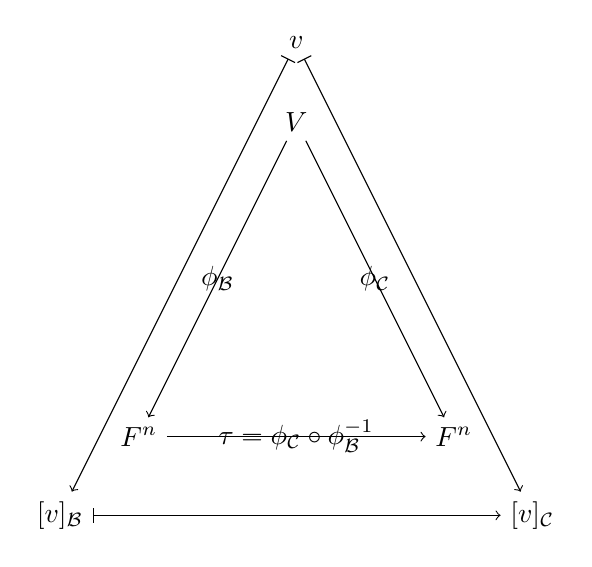
\begin{tikzpicture}
        \node(1)at(0,2){$V$};
        \node(2)at(-2,-2){$F^n$};
        \node(3)at(2,-2){$F^n$};
        \node(4)at(0,3){$v$};
        \node(5)at(-3,-3){$[v]_{\mathcal{B}}$};
        \node(6)at(3,-3){$[v]_{\mathcal{C}}$};
        \draw[->](1)--(2)node[midway]{$\phi_{\mathcal{B}}$};
        \draw[|->](4)--(5);
        \draw[->](1)--(3)node[midway]{$\phi_{\mathcal{C}}$};
        \draw[|->](4)--(6);
        \draw[->](2)--(3)node[midway]{$\tau=\phi_{\mathcal{C}}\circ\phi_{\mathcal{B}}^{-1}$};
        \draw[|->](5)--(6);
    \end{tikzpicture}
\end{center}

$[v]_{\mathcal{C}}=\tau([v]_{\mathcal{B}})=M_{\tau}[v]_{\mathcal{B}}$, 其中 $M_{\tau}=\begin{pmatrix}
    \tau(e_1)&\cdots&\tau(e_n)
\end{pmatrix}$.\\
$\tau:F^n\rightarrow F^n,\quad e_i\mapsto\tau(e_i)=\phi_{\mathcal{C}}(\phi_{\mathcal{B}}^{-1}(e_i))=\phi_{\mathcal{C}}(b_i)$,\\
$M_{\tau}=\begin{pmatrix}
    [b_1]_{\mathcal{C}}&\cdots&[b_n]_{\mathcal{C}}
\end{pmatrix}\equiv M_{\mathcal{BC}}$.

\begin{thm}[(课本定理 2.12)]
    \begin{align*}
        \boxed{[v]_{\mathcal{C}}=M_{\mathcal{BC}}[v]_{\mathcal{B}}}
    \end{align*}
    其中 $[v]_{\mathcal{B}}$ 和 $[v]_{\mathcal{C}}$ 分别是向量 $v$ 在基 $\mathcal{B}$ 和 $\mathcal{C}$ 表象下的坐标表示, $M_{\mathcal{BC}}$ 是在两种坐标表示之间线性变换对应的矩阵.
\end{thm}

\begin{center}
    \begin{tikzpicture}
        \node(1)at(-2,2){$V$};
        \node(2)at(2,2){$W$};
        \node(3)at(-2,-2){$F^n$};
        \node(4)at(2,-2){$F^n$};
        \node(5)at(-3,3){$v$};
        \node(6)at(3,3){$\tau(v)$};
        \node(7)at(-3,-3){$[v]_{\mathcal{B}}$};
        \node(8)at(3,-3){$\tau([v]_{\mathcal{B}})=[v]_{\mathcal{C}}$};
        \node(9)at(-4,4){$b_i$};
        \node(10)at(4,4){$\tau(b_i)$};
        \node(11)at(-4,-4){$e_i$};
        \node(12)at(4,-4){$\tau_A(e_i)=[\tau(b_i)]_{\mathcal{C}}$};
        \draw[->](1)--(2)node[midway]{$\tau$};
        \draw[->](1)--(3)node[midway]{$\phi_{\mathcal{B}}$};
        \draw[->](2)--(4)node[midway]{$\phi_{\mathcal{C}}$};
        \draw[->](3)--(4)node[midway]{$\tau_A=\phi_{\mathcal{C}}\circ\tau\circ\phi_{\mathcal{B}}^{-1}$};
        \draw[|->](5)--(6);
        \draw[|->](5)--(7);
        \draw[|->](6)--(8);
        \draw[|->](7)--(8);
        \draw[|->](9)--(10);
        \draw[|->](9)--(11);
        \draw[|->](10)--(12);
        \draw[|->](11)--(12);
    \end{tikzpicture}
\end{center}
\begin{align*}
    M_{\tau_A}=&\begin{pmatrix}
        \tau_A(e_1)&\cdots&\tau(e_n)
    \end{pmatrix}=\begin{pmatrix}
        \phi_{\mathcal{C}}\circ\tau\circ\phi_{\mathcal{B}}^{-1}(e_1)&\cdots&\phi_{\mathcal{C}}\circ\tau\circ\phi_{\mathcal{B}}^{-1}(e_n)
    \end{pmatrix}=\begin{pmatrix}
        \phi_{\mathcal{C}}\circ\tau(b_1)&\cdots&\phi_{\mathcal{C}}\circ\tau(b_n)
    \end{pmatrix}\\
    =&\begin{pmatrix}
        [\tau(b_1)]_{\mathcal{C}}&\cdots&[\tau(b_n)]_{\mathcal{C}}
    \end{pmatrix}\equiv[\tau]_{{\mathcal{BC}}}.
\end{align*}

\begin{thm}[(课本定理 2.14)]
    \begin{align*}
        \boxed{[\tau(v)]_{\mathcal{C}}=[\tau(v)]_{\mathcal{BC}}[v]_{\mathcal{B}}}
    \end{align*}
    其中 $[\tau(v)]_{\mathcal{C}}$ 是 $\tau(v)$ 在基 $\mathcal{C}$ 的表象下的坐标表示, $[\tau(v)]_{\mathcal{BC}}$ 是从基 $\mathcal{B}$ 的表象到基 $\mathcal{C}$ 的表象的线性变换的矩阵表示, $[v]_{\mathcal{B}}$ 是 $v$ 在基 $\mathcal{B}$ 的表象下的坐标表示.
\end{thm}

\begin{thm}[(课本定理 2.15)]
    $\mathcal{L}(V,W)\rightarrow\mathcal{L}(F^n,F^m)\approx M_{m\times n}(F)$, $\tau\mapsto\tau_A\mapsto[\tau]_{\mathcal{BC}}$.
\end{thm}

若我们改变 $V$ 和 $W$ 的基, 那么映射所联系的向量的坐标会如何?

\begin{center}
    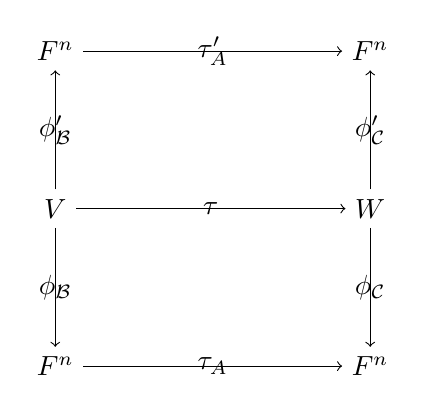
\begin{tikzpicture}
        \node(1)at(-2,0){$V$};
        \node(2)at(2,0){$W$};
        \node(3)at(-2,-2){$F^n$};
        \node(4)at(2,-2){$F^n$};
        \node(5)at(-2,2){$F^n$};
        \node(6)at(2,2){$F^n$};
        \draw[->](1)--(2)node[midway]{$\tau$};
        \draw[->](1)--(3)node[midway]{$\phi_{\mathcal{B}}$};
        \draw[->](2)--(4)node[midway]{$\phi_{\mathcal{C}}$};
        \draw[->](3)--(4)node[midway]{$\tau_A$};
        \draw[->](1)--(5)node[midway]{$\phi_{\mathcal{B}}'$};
        \draw[->](2)--(6)node[midway]{$\phi_{\mathcal{C}}'$};
        \draw[->](5)--(6)node[midway]{$\tau_A'$};
    \end{tikzpicture}
\end{center}

$\tau_A'=\phi_{\mathcal{C}}'\phi_{\mathcal{C}}^{-1}\tau_A\phi_{\mathcal{B}}\phi_{\mathcal{B}}'^{-1}$.

\begin{thm}[(课本定理 2.16)]
    \begin{align*}
        \boxed{[\tau]_{\mathcal{B'C'}}=M_{CC'}[\tau]_{\mathcal{BC}}M_{\mathcal{B'B}}}
    \end{align*}
    其中 $[\tau]_{\mathcal{BC}}$ 和 $[\tau]_{\mathcal{B'C'}}$ 分别是线性变换 $\tau$ 在基 $(\mathcal{B},\mathcal{C})$ 和 $(\mathcal{B}',\mathcal{C}')$ 下的表示, 矩阵 $M_{\mathcal{B'B}}$ 和 $M_{\mathcal{CC}'}$ 分别对应了从基 $\mathcal{B}$ 到基 $\mathcal{B}'$ 和从基 $\mathcal{C}$ 到基 $\mathcal{C}'$ 的变换矩阵.
\end{thm}

$M_{\mathcal{BB}'}$ 可逆.
\begin{pf}
    设 $\phi_{\mathcal{B}}:V\rightarrow F^n$, $v=\sum_{i=1}^nr_ib_i\mapsto[v]_{\mathcal{B}}=\begin{pmatrix}
        r_1\\
        \vdots\\
        r_n
    \end{pmatrix}$ , $\phi_{\mathcal{B}'}:V\rightarrow F^n$, $v=\sum_{i=1}^nr_i'b_i'\mapsto[v]_{\mathcal{B}'}\begin{pmatrix}
        r_1'\\
        \vdots\\
        r_n'
    \end{pmatrix}$, 即
    \begin{center}
        \begin{tikzpicture}
            \node(1)at(0,2){$V$};
            \node(2)at(-2,-2){$F^n$};
            \node(3)at(2,-2){$F^n$};
            \node(4)at(0,3){$v$};
            \node(5)at(-3,-3){$[v]_{\mathcal{B}}$};
            \node(6)at(3,-3){$[v]_{\mathcal{B}'}$};
            \draw[->](1)--(2)node[midway]{$\phi_{\mathcal{B}}$};
            \draw[->](1)--(3)node[midway]{$\phi_{\mathcal{B}'}$};
            \draw[->](2)--(3)node[midway]{$\tau$};
            \draw[|->](4)--(5);
            \draw[|->](4)--(6);
            \draw[|->](5)--(6);
        \end{tikzpicture}
    \end{center}
    $M_{\mathcal{BB}'}=M_{\tau}=\begin{pmatrix}
        [b_1]_{\mathcal{B}'}&\cdots&[b_n]_{\mathcal{B}'}
    \end{pmatrix}$, s.t. $[v]_{\mathcal{B}'}=M_{\mathcal{BB}'}[v]_{\mathcal{B}}$.\\
    同理可以构造 $M_{\mathcal{BB}'}=\begin{pmatrix}
        [b_1']_{\mathcal{B}}&\cdots&[b_n']_{\mathcal{B}}
    \end{pmatrix}$, s.t. $[v]_{\mathcal{B}}=M_{\mathcal{B'B}}[v]_{\mathcal{B}'}$.\\
    $\forall[v]_{\mathcal{B}}\in F^n$, $M_{\mathcal{BB}'}M_{\mathcal{B'B}}[v]_{\mathcal{B}}=M_{\mathcal{BB}'}[v]_{\mathcal{B}'}=[v]_{\mathcal{B}}\Longrightarrow M_{\mathcal{BB}'}M_{\mathcal{B'B}}=n\times n$ 维的单位矩阵, 即 $M_{\mathcal{B'B}}$ 是 $M_{\mathcal{BB}'}$ 的逆, 故 $M_{\mathcal{BB}'}$ 可逆.
\end{pf}

\begin{thm}[(课本定理 2.18)]
    $B=PAQ$, 其中 $P$ 和 $Q$ 可逆, 则 $B$ 与 $A$ \textbf{等价}.
\end{thm}
(因为 $B$ 和 $A$ 是同一线性变换在两组不同的基下的表示.)

\begin{thm}[(课本定理 2.19)]
    $B=PAP^{-1}$, 其中 $P$ 可逆, 则 $B$ 与 $A$ \textbf{相似}.
\end{thm}
(因为 $B$ 和 $A$ 是同一线性算子在两组不同的基下的表示.)
\ifx\allfiles\undefined
\end{document}
\fi